\documentclass[../thesis.tex]{subfiles}

\begin{document}

\chapter{Event selection}
\label{chap:selection}

% XXX See Kam-Biu's initial comment. Need plots/tables showing the effect of each cut. Also add a plot/flowchart for DQ shift process. Maybe a screenshot?

From the sequence of reconstructed triggers in the ADs, we are primarily interested in extracting IBD candidates, in order to obtain the antineutrino rate and spectrum. The tight time correlation of the prompt and delayed triggers, as well as the relatively high 8~MeV energy released from the nGd capture, enable the extraction of a $\sim$98\% pure sample of IBDs, from which the independently estimated backgrounds can then be subtracted.

Aside from the IBD selection, this analysis also employs an extraction of \emph{singles,} that is, those events that produce only a single trigger, uncorrelated in time with any others. The purpose of the singles sample is to enable determination, firstly, the rate and spectrum of backgrounds produced by accidental coincidences, and secondly, the efficiency of the multiplicity cut (discussed in \autoref{sec:pairSel}).

Both selections are implemented using a two-stage approach. In the first stage, the \emph{pre-selection,} processed (i.e., calibrated and reconstructed) Daya Bay data files are scanned, unimportant events are ignored, and of the remaining events, only the minimum required data fields are stored in the output. This process reduces $\sim$600,000 input files (each representing $\sim$10 minutes of data collection), totaling some 600~TB, down to about 5,500 files (each representing one hall $\times$ day), totaling one terabyte. In the second stage, the \emph{final selection,} the full set of selection criteria are applied to the pre-selected data, producing samples of IBDs and singles for use in the oscillation analysis. This two-stage approach significantly reduces the amount of time needed to generate new IBD/singles samples after modifying the selection criteria, since the pre-selection does not need to be re-run. When the NERSC cluster is not under severe disk I/O load, the two-stage approach provides a speed improvement of 3 to 4; during disk overload, the improvement can be greater still.

\section{Data production}
\label{sec:selProd}

The IBD and singles selection do not proceed directly from the raw Daya Bay data files, but instead from the processed files produced during \emph{data production}, in which the previously-discussed steps of calibration and reconstruction are applied. We briefly describe the production process here. For the data sample used in this analysis, production was largely conducted and monitored by the author. This was the first time that production was performed on the high-performance computing (HPC) systems at the National Energy Research Scientific Computing Center (NERSC). To achieve this milestone, nontrivial changes to the production infrastructure were required, and new scripts and tools had to be developed.

Production begins with the raw data files produced by Daya Bay's onsite data acquisition (DAQ) software. We will refer to these as ``DAQ files''. The DAQ files, which use a specialized binary file format, contain the ADC count (and pedestal) and TDC count for each PMT hit in a given trigger, as well as the global details of each trigger, such as the detector, timestamp, and trigger type. Although each hall as its own DAQ system, the subdetectors within each hall (ADs, WPs, and RPCs) are all read out by the same DAQ. Each DAQ file thus contains all of the data generated by a given hall within a given time period. The DAQs are configured to output a new file after approximately 1~GB of data has been accumulated, corresponding to about 10~minutes in the near halls and 20~minutes in EH3. Each DAQ file is identified by its \emph{run number}\footnote{Run numbering is sequential, and all three halls share the same global counter; that is, there is no possibility of two runs in different halls sharing the same run number.} and \emph{file number} (starting at 1 and increasing sequentially within each run).

During production, each DAQ file is independently processed by Daya Bay's offline software framework, NuWa, which is based on the Gaudi \cite{gaudi} framework used by various other experiments, including the LHC's ATLAS. NuWa was developed by extending Gaudi with various algorithms, services, and tools that serve such purposes as parsing the DAQ file format, outputting the ROOT file format, and performing calibration, reconstruction, and event tagging. For each DAQ file, NuWa produces a corresponding ROOT file containing, for each trigger the calibrated charge and time of each PMT hit, the total nominal charge, the reconstructed energy and vertex, and numerous other useful high-level quantities. In addition, the output file contains tags that identify potential muons, coincidence pairs, isolated single events, etc., although these tags are generally not employed in this analysis.\footnote{However, tagged muon-like events are used in our characterization of the $^9$Li/$^8$He background, as discussed in \autoref{sec:bkgLi9MuonSel}.}

Previous data productions ran on NERSC's older (non-HPC) Parallel Distributed Systems Facility (PDSF), on which each file was processed by a separate batch job (using Univa Grid Engine, now Altair Grid Engine \cite{AltairGridEngine}) on the cluster. However, for the HPC systems (Cori and Edison), a considerably more complex scheme was necessary in order to harness the full performance potential of the facilities. In particular, due to the large number of parallel jobs, it was no longer possible to point them all toward a single instance of the Daya Bay offline database (containing calibration constants, etc.), as doing so was guaranteed to overload the database. Furthermore, effective use of the HPC system required using long-running jobs in which each allocated core would need to process multiple files sequentially, a significant deviation from the previous technique of pre-assigning a single DAQ file to each job.

Accordingly, for the HPC systems (based on SLURM \cite{SLURM} instead of Univa Grid Engine), the production system was completely overhauled. First, the list of DAQ files was loaded into a RabbitMQ \cite{RabbitMQ} queue. Then, instead of having each job process a single file on a single core, with a single central database, we opted to submit SLURM jobs which each requested a few dozen compute nodes (with the exact number depending on the particular system used). Using Shifter container technology \cite{shifter}, a clone of the offline database was provisioned (on one node) for each job. On the remaining nodes for each job, a few dozen parallel \emph{pilot tasks} were launched (again using Shifter to provide the correct software environment for NuWa), limited by the available amount of memory.\footnote{Due to NuWa's high memory requirements, memory was the bottleneck, rather than the number of CPU cores.} Each pilot task then repeatedly queried the RabbitMQ queue for DAQ files to process, continuing until the job's time limit approached.

This system was successful in scaling up Daya Bay's data production in order to harness the power of NERSC's HPC facilities. Using a small fraction of the total system capacity, this data production was completed in approximately a week, with a shorter turnaround easily obtainable had a larger allocation been given. The previous production system would have taken more than a month. The infrastructure developed for this production continues to be used for high-throughput processing of Daya Bay's data.

Once each file has been processed and validated, the resulting ROOT file is stored and cataloged for use in analysis. It is these files that we use in selecting IBDs and singles for this analysis.

\section{IBD selection}
\label{sec:selIBDs}

We begin by discussing the IBD selection. The singles selection proceeds similarly, with minor differences in the final steps, as discussed in \autoref{sec:selSingles}.

\subsection{Pre-selection}
\label{sec:selPreSel}

\subsubsection{Input data}
\label{sec:selInputData}

The processed (i.e. reconstructed) Daya Bay files (in ROOT format) serve as the input to the pre-selection. Although these files contain basic taggings of muon-like events and coincidence clusters, this information is not used here; our event selection is a completely independent implementation.

Two ROOT TTrees are read in parallel: the \texttt{AdSimple} tree, which contains the reconstructed energy, and the \texttt{CalibStats} tree, which contains the nominal charge (used, in some cases, for pre-muon%
\footnote{The meaning of \emph{pre-muon} is explained below, in the section labeled \emph{Pre-muon selection.}}
% \footnote{We define a \emph{pre-muon} as any AD event with more than 3,000~pe of nominal charge, or any WP event with more than 12 hit PMTs. For the nominal IBD selection, these definitions correspond to those of AD and WP muons, respectively. The name \emph{pre-muon} highlights the fact that we are free, in later stages of the analysis, to define our actual muon vetos differently, e.g., requiring an AD muon to have a charge of at least 5,000~pe.}
identification in the ADs), the number of hit PMTs (ignored for AD events, but used for identifying pre-muons in the water pool), and various quantities that are used for removing instrumental backgrounds. Both trees are of the same length, with one entry per trigger, including triggers in the water pools and RPCs (for which AD-specific quantities are left blank). Being the same length, the two trees can be ``friended'' together (in ROOT parlance) and scanned as one. Other fields loaded from this combined tree are the detector ID, the trigger type, the trigger ID, and the trigger time.

\subsubsection{Trigger type restriction}
\label{sec:selTrigType}

The very first criterion applied in the pre-selection is a restriction on the type of triggers saved. In particular, six types of triggers are excluded: manual triggers, cross triggers (issued when a trigger occurs in a different detector subsystem), periodic and random triggers (used for subthreshold and noise measurements), pedestal triggers (used in special runs to measure the ADC pedestals), and calibration triggers (issued, for instance, when a calibration LED is pulsed). The remaining events consist solely of \texttt{NHit} and \texttt{ESum} triggers, issued (respectively) when the number of hit channels or the total measured charge, within the previous \us, is above a configured threshold. The NHit threshold is 45, while the ESum threshold (in units roughly, but not exactly, analogous to the nominal charge) is 100, 107, and 130 in EH1, EH2, and EH3 (corresponding roughly to 0.63, 0.67, and 0.81~MeV, respectively\footnote{Even though the EH3 ESum threshold may appear to lack perfect efficiency at 0.7~MeV, the NHit condition, along with the subtle differences between the (hardware) ESum and the (software) nominal charge, ensure near-100\% efficiency at 0.7~MeV. Indeed, the NHit trigger alone reaches 100\% efficiency at 0.5~MeV \cite{weili_trig_eff}}.). These thresholds were determined during commissioning in order to ensure perfect trigger efficiency at the IBD prompt energy threshold of 0.7~MeV, without overwhelming the trigger rate.

\subsubsection{Pre-muon selection}
\label{sec:selPreMuons}

After removing unwanted trigger types, the next step in the pre-selection is to extract muon-like events to an output tree of \emph{pre-muons.} The actual definition of a muon (for the purpose of applying the muon veto) is applied in stage two; the pre-muon criteria are thus designed to be loose enough to encompass any final muon definition. An event in the water pool is considered a pre-muon if the number of hit PMTs is more than 12,%
\footnote{Any PMT with at least one hit recorded in the readout, regardless of location in time relative to the trigger, is included in the \texttt{CalibStats} count of hit PMTs, for both the water pools and the ADs, although we do not use the hit count in the latter case.}%
and an AD pre-muon is defined as having a nominal charge of more than 3,000 photoelectrons.
%\footnote{In previous versions of the pre-selection, AD pre-muons were defined in terms of nominal charge rather than energy, with a cut at 3,000 p.e. This was done for the sake of consistency with the original LBNL IBD selection, which defined muons in terms of charge rather than energy. However, the uniform use of energy simplifies matters somewhat, so this departure was made from the original selection.}
Each pre-muon was stored with its trigger time and its \emph{strength}, either its nominal charge (for AD triggers) or its hit multiplicity (for WP triggers).

\subsubsection{Flasher removal}
\label{sec:selFlashers}

Among the remaining non-pre-muon events, some are \emph{flashers,} instrumental backgrounds produced by arcing within the base of the PMTs. The light from these arcs can illuminate the detector, resulting in a trigger. As detailed in \autoref{sec:bkgFlashers}, these events can be easily distinguished by their characteristic conical pattern of light emission. The three cuts described in \autoref{sec:bkgFlashers} (the \emph{ellipse,} \emph{PSD,} and \emph{2" PMT} cuts) are used to identify and remove flashers from the output.

\subsubsection{Saving and merging}
\label{sec:selMergingOne}

Finally, the non-pre-muon, non-flasher triggers are saved in their own tree (one for each AD), separate from the pre-muon tree. For each event, the run number, file number, trigger time, trigger number, and energy are saved. A minimum reconstructed energy of 0.7~MeV (the threshold for prompt-like triggers) is applied here to further reduce the data volume, since lower-energy events are not considered in this analysis.

The pre-selection files are initially produced in one-to-one correspondence with the reconstructed DAQ files, resulting in $\sim$600,000 small files. To reduce the file count and improve IO performance, these files are merged (using ROOT's \texttt{hadd}) into files that each represent one calendar day in one hall, a total of $\sim$5,500 files. Finally, these daily files are pre-loaded into a solid-state device \emph{burst buffer} at the National Energy Research Scientific Computing Center (NERSC), to ensure that the performance of the final selection will be minimally impacted by disk load conditions at the facility.

\subsection{Final selection}
\label{sec:selFinalSel}

The specific thresholds for the cuts described in this section are \emph{nominal}; they are defined somewhat arbitrarily based on qualitative observations and notions of reasonableness, intended to give a satisfactory ratio of signal to background. Later, in \autoref{chap:cutVary}, we study the effects of varying these cuts, with the aim of jointly optimizing both the uncertainty on the oscillation parameters as well as the stability of the fit with respect to variations in the cuts. Doing so will eliminate the arbitrariness inherent in the cuts described here.

\subsubsection{Muon veto}
\label{sec:selMuonVeto}

When a muon passes through or near the AD, it can produce triggers in the aftermath. These can include instrumentally-induced triggers (caused by PMT afterpulsing and electronics ringing in the 20~\us\ following the muon \cite{Jetter_2012}), as well as physical events. The physical events can include spallation neutrons, whose thermalization and subsequent capture can mimic an IBD, isotopes such as $^9$Li, and $^8$He, which produce neutrons when they decay, and various uncorrelated decays that can form accidental IBD-like pairs.

For this reason, it is essential to veto the time period immediately following a muon. Although the mean neutron capture time in the GdLS is only 28~\us, neutrons can be produced outside the GdLS and slowly diffuse into it, necessitating a significantly longer veto window. In the case of muons passing through the water pools (``WP muons''), a veto time of 600~\us\ was shown to effectively remove all such neutrons. Only relatively energetic neutrons, i.e. fast neutrons, would have the ability to reach the GdLS; diffusion from the WP to the GdLS, meanwhile, is not a significant possibility for thermal neutrons produced by WP muons. Meanwhile, for muons passing through the ADs (``AD muons''), neutrons \emph{can} diffuse slowly from the LS or mineral oil, leading to the requirement of a veto window closer to a millisecond. The nominal window for this case is 1.4~ms, a factor of $\sim$7 larger than the mean neutron capture time (mainly on hydrogen) in the LS region. AD muons are nominally defined as those triggers having a nominal charge of at least 3,000~photoelectrons.

Muons that deposit an especially high amount of energy in the AD are termed \emph{shower} muons. Compared to lower-energy (i.e., minimum ionizing) muons, shower muons have a much higher probability of producing the two cosmogenic isotopes $^9$Li and $^8$Be, discussed further in \autoref{sec:bkgCosmo}. These isotopes undergo beta decay, producing a prompt-like trigger, and then break up to produce neutrons which are captured, producing a delayed-like trigger. Given that the lifetime of these isotopes is of order 100~ms, the ordinary AD muon veto of around one millisecond would fail to significantly reduce these backgrounds. Accordingly, a much longer veto window is needed after a shower muon. The nominal window is 1~s, with shower muons defined as having an energy of at least 2~GeV. At this threshold energy, the rate of $^9$Li/$^8$He production is low enough to avoid backgrounds from sub-threshold muons, while the rate of such muons themselves is also low enough to avoid too large of a loss in effective detector livetime. These qualititative statements are refined more quantitatively in \autoref{chap:cutVary}, where we explore the effects of modifying the muon veto thresholds and windows.

An additional veto window is applied, spanning 2~\us\ \emph{before} each muon, common to the WP, AD, and shower muons. Given that trigger latencies can vary, it is possible for a WP muon trigger to receive a trigger timestamp that comes \emph{after} the timestamps for muon-induced events in the AD. The 2~\us\ pre-veto eliminates this possibility. There is no particular need to veto the 2~\us\ preceding an \emph{AD} muon, but the original LBNL IBD selection did so anyway, and we honor its legacy by following suit.\footnote{As discussed in \autoref{chap:accDMC}, an enlarged pre-veto of 200~\us\ provides a more rigorous mathematical decoupling of the muon veto and multiplicity cut efficiencies, but the practical advantage of this is negligible.}

During application of the muon veto, the total amount of vetoed time is tracked, accounting for overlaps. This value is used in order to calculate the muon veto efficiency, determined (on a daily basis) simply as the ratio of unvetoed DAQ livetime to total DAQ livetime. It should be noted that the muon veto is only applied to the \emph{delayed} trigger of a coincidence pair, and this is what enables the efficiency to be calculated so simply. Otherwise, we would require a complex calculation involving the prompt-delayed time distribution and the muon rate. Given (as described below) that the maximum time difference between the prompt and delayed event is 200~\us, it is possible for the prompt trigger to lie 200~\us\ before the end of the veto window. The windows are thus made large enough to ensure that this time period is free of muon-correlated activity. An illustration of the three muon vetoes is provided in \autoref{fig:veto_diagram_rM}.

\begin{figure}[h!]
  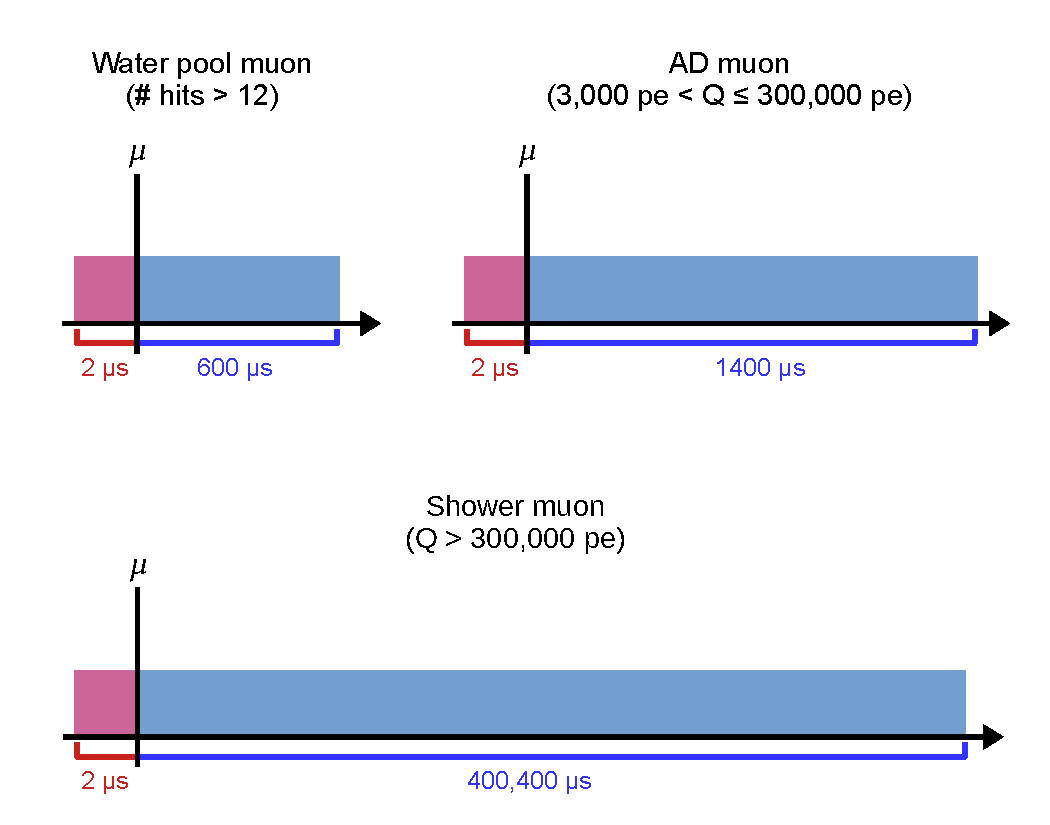
\includegraphics[width=0.8\textwidth]{Selection/veto_diagram_new.pdf}
  \caption{Illustration of the muon veto scheme. The purple (pink) shaded region is the vetoed time after (before) the muon. Not to scale.}
  \label{fig:veto_diagram_rM}
\end{figure}

\subsubsection{Pair selection}
\label{sec:pairSel}

A potential IBD candidate may be lurking whenever there is a non-vetoed delayed-like trigger (i.e., one lying between 6 and 12~MeV). Specifically, the following conditions (known as the \emph{decoupled}\footnote{The meaning of ``decoupled'' is explained further in \autoref{chap:accDMC}.} \emph{multiplicity cut}, or DMC) determine the existence of an IBD candidate (\autoref{fig:dmc_diagram_rM}):

\begin{enumerate}
\item There is a prompt-like (i.e. 0.7--12~MeV) trigger between 1 and 200~\us\ before this delayed-like trigger
\item There are no other triggers of more than 0.7~MeV between 1 and 400~\us\ before this delayed-like trigger.\footnote{Originally, this condition was framed in terms of \emph{prompt-like}, rather than $>$0.7~MeV triggers, but the permitted ``extra'' events above 12~MeV (i.e. low-energy muons) were found to be correlated with backgrounds consisting of pairs of neutron captures. The modified condition eliminates this background.}
\item There are no delayed-like triggers within 200~\us\ after this one.
\end{enumerate}

\begin{figure}[h]
  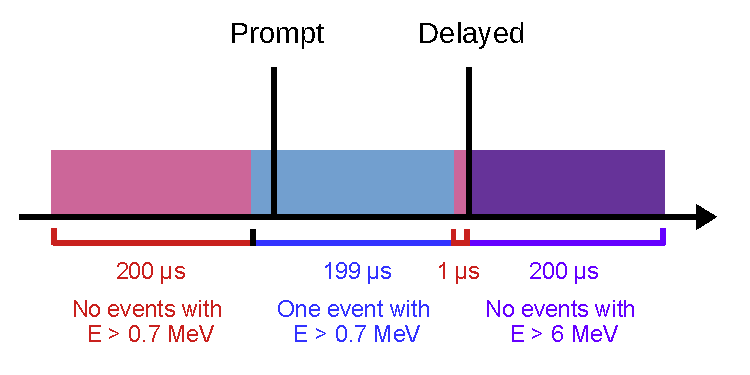
\includegraphics[width=0.7\textwidth]{Selection/dmc_diagram_new.pdf}
  \caption{Illustration of the decoupled multipicity cut. The blue region must contain exactly one prompt-like event, the pink regions must contain no prompt-like events, and the purple region must contain no delayed-like events. Not to scale.}
  \label{fig:dmc_diagram_rM}
\end{figure}

The purpose of the latter two conditions is to avoid the ambiguity that can arise, for instance, in the contrived example of three 7~MeV events spaced 100~\us\ apart. Here there are three possible ways to form a pair. There are other possible ways to define cuts that would avoid this ambiguity, for instance, by defining ``empty'' windows relative to the prompt trigger, but the DMC allows for a simple calculation of the efficiency as well as an avoidance of correlations with the muon veto efficiency, as described in \autoref{chap:accDMC}.

IBD candidates that pass the DMC are stored in an output tree containing the run and file number, the prompt-delayed time difference, and the IDs and energies of the two triggers.

\subsubsection{Merging and post-processing}
\label{sec:selMergingTwo}

After the $\sim$5,500 hall-daily files have been fully produced, they are merged with \texttt{hadd} into nine files, the product of three halls and three periods (the 6AD, 8AD, and 7AD periods, whose names reference the number of operating ADs). The splitting into periods is done for convenience in preparing the input files required by the fitter, which expects separate files for each period. The fitter's input files, which consist of the IBD spectra, the accidentals spectra, and textual tables of rates, efficiencies, backgrounds, uncertainties, etc., are prepared by a simple script from these nine hall-period files.

\subsubsection{Extracted prompt spectra}
\label{sec:selPromptSpec}

Altogether, these steps produce a set of IBD candidates (including backgrounds) for each AD. The prompt energies of these candidates are then used to generate the prompt spectra (in the form of histograms) \autoref{fig:selPromptSpec} shows the total prompt spectrum for each hall obtained using the nominal IBD selection cuts. Although backgrounds have not been subtracted, the total relative background rate at Daya Bay is only 1--2\%, so these spectra provide a reasonable measurement of the true IBD spectral shape, and will be referenced for this purpose throughout this text.

\begin{figure}[h]
  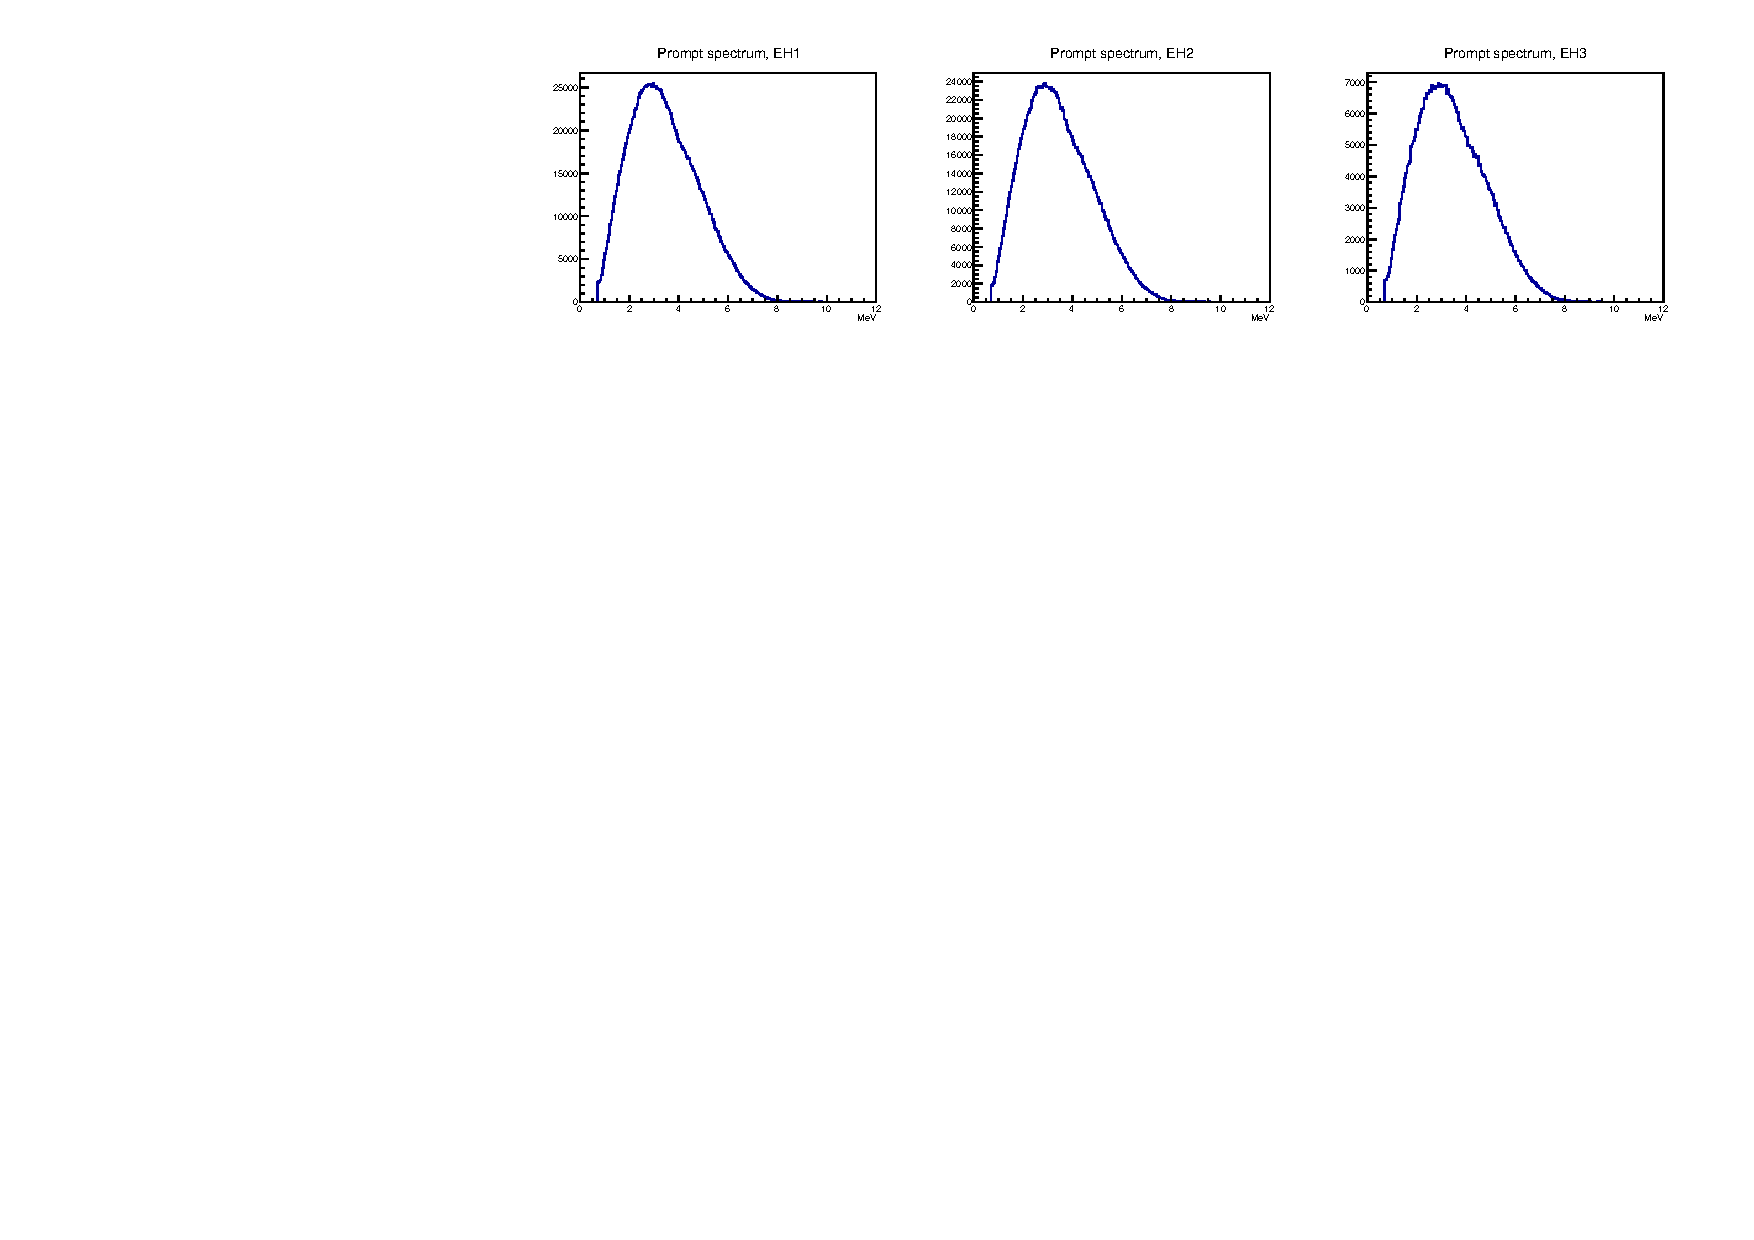
\includegraphics[scale=0.8]{Selection/prompt_spec_3halls.pdf}
  \caption{Reconstructed prompt energy of the nominal set of IBD candidates for each hall.}
  \label{fig:selPromptSpec}
\end{figure}

\section{Singles selection}
\label{sec:selSingles}

The singles selection proceeds in a similar manner to the IBD selection, except that pairs are no longer being selected. Instead, when a non-muon trigger of at least 0.7~MeV is found, an \emph{isolation cut} is applied, eliminating those events for which another 0.7~MeV trigger lies within specified windows before and after the ``singles candidate''. As implemented, the windows used are 400~\us\ before the trigger and 200~\us\ after, chosen to resemble the DMC as closely as possible. In principle, the exact sizes of these windows should not matter (provided they are wide enough to eliminate correlated multiplets), as the efficiency of the isolation cut is corrected for in calculating the DMC efficiency and accidental background rate. In practice, due to correlated low-energy processes such as alpha-alpha and beta-alpha cascades (from, e.g., Bi-Po decays in the decay chains of actinides, as considered in \autoref{sec:bkgCanO}), the singles sample does not fully consists of ``true'' singles, so the choice of DMC-like time windows is a naive attempt to minimize any resulting biases. Ultimately, the uncertainty of the accidental background rate is inflated beyond the statistical uncertainty in order to account for this problem.

\section{Data quality}
\label{sec:selDataQuality}

In order to avoid potential biases on the extracted oscillation parameters, it is essential that data only be used from periods when the detectors are behaving as designed. From time to time, hardware might malfunction, runs might be misconfigured, or calibrations may be erroneous, resulting in questionable data quality. Accordingly, Daya Bay features a comprehensive program of data quality monitoring, review, and recordkeeping. These activities, carried out by the Data Quality Working Group (DQWG), culminate in the publication of ``good run lists'' (technically, good \emph{file} lists) which specify those data files that are suitable for use in physics analysis.

Daya Bay's first line of defense against bad data is made up of ``shifters'', ordinary collaborators carrying out their obligation to occasionally take 8-hour shifts monitoring the experiment. At any given time, there is at least one shifter on duty, who periodically carries out a checklist to verify that the experiment is operating normally. This procedure includes checking for any alarms from the Detector Control System, which monitors environmental parameters (temperature, humidity, etc.), liquid levels, PMT high voltages, and various mechanical and electronic systems. Aside from the alarms, a number of plots are also checked by the shifter. These plots show various quantities (such as PMT hit rates and average pulse sizes, trigger rates and trigger types, and overall data rates), comparing the current values to those from ``normal'' historical data.

If any possible issues are noticed, the shifter records a note in the logbook and notifies the designated experts for the subsystem in question. The experts may then contact the DQWG to report a potential data quality issue. Alternatively, the shifter may submit a report directly to the DQWG either via email or a web form. In addition to receiving such reports, the DQWG also monitors the shift logbook to see whether the shifters have noted anything worthy of further investigation.

Data quality records, such as the aforementioned reports from shifters, are maintained in a Data Quality Database (DQDB). The DQDB also stores the quality rating (i.e., good, bad, or to-be-determined) of each data file, along with a reference to a comment record that describes the reason why a file has been ``tagged'' as bad. Finally, the DQDB stores various physics-driven metrics for each file (such as event rates and peak energies), which are utilized in the procedures carried about by the DQ shifter, as described later.

The DQ metrics are calculated and recorded at IHEP during Keep Up Production (KUP), in which Daya Bay's data production software (which carries out calibration, reconstruction, tagging, etc.) is automatically run on each new raw data file received from onsite. During KUP, calibration is performed using the ``old'' constants from the end of the previous data production, so the results are not suitable for precise analysis, but they suffice for monitoring detector stability and sanity.

For each detector, the KUP software calculates the rates of various event classes (overall triggers, prompt-like events, $^{40}$K events, etc.), the energies of various peaks ($^{40}$K, n-Gd capture, etc.), and the rate of infrequent blocked triggers (caused by excessive pileup, typically by noise in the electronics). These quantities are then uploaded to the DQDB for use by external tools employed by DQ shifters and the DQWG.

The review of these metrics is the responsibility of the DQ shifter, Daya Bay's second line of defense. The DQ shifter uses the DQ shift website to view time series plots of one or more selected metrics (\autoref{fig:selDybvdqShot}). All metrics, and all detectors in a given hall, are shown on the same page. Under general circumstances, the DQ shifter typically looks at the prompt-like rate, the $^{40}$K peak energy, and the AD and WP blocked trigger rates, since the vast majority of data quality issues will manifest themselves in at least one of these plots.

\begin{figure}[h!]
  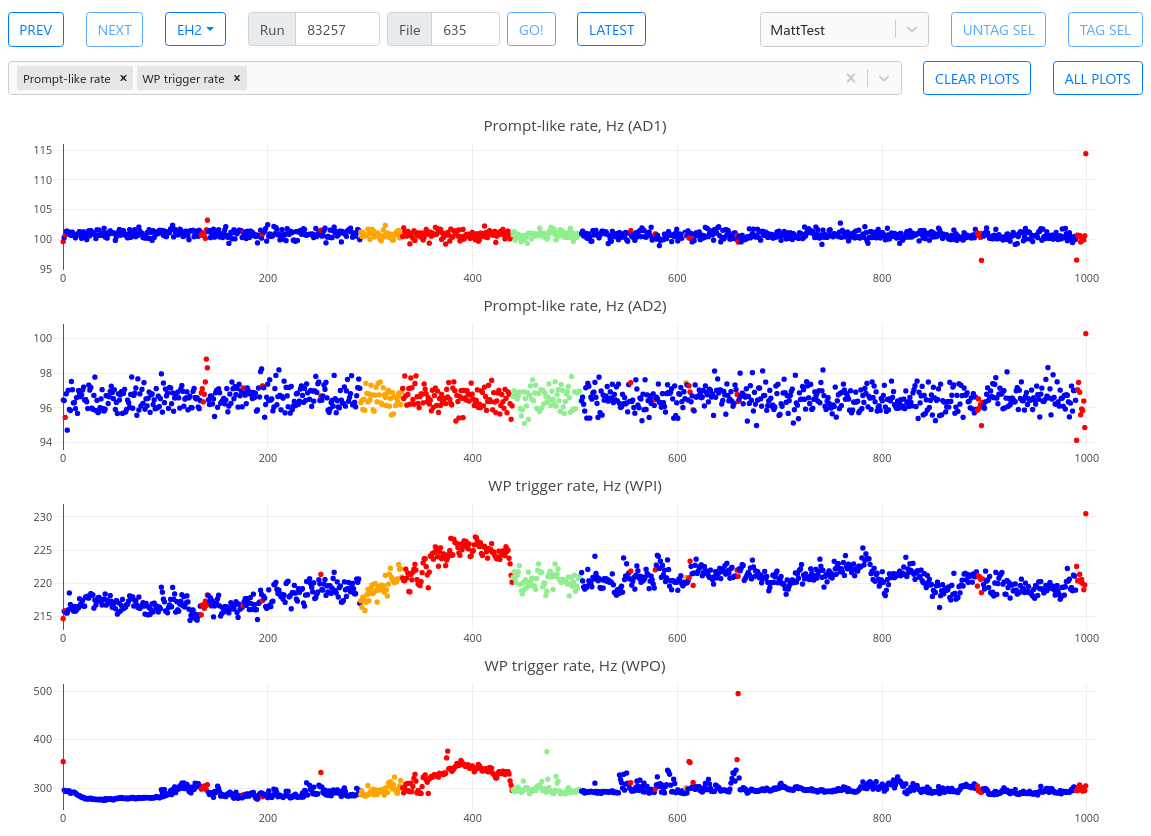
\includegraphics[width=\textwidth]{Selection/dybvdq_shot.png}
  \caption[Screenshot of Daya Bay data quality website.]{Screenshot of the Daya Bay data quality shift website, developed by the author \cite{dybvdq}. Each point represents a data file; each plot represents a quantity of interest. Blue points are good (untagged) files; red points are files tagged as bad; orange points are files proposed for tagging as bad; green points are tagged files proposed for untagging.}
  \label{fig:selDybvdqShot}
\end{figure}

Any abnormal data points (i.e. files) can be clicked on by the DQ shifter; this will ``locally'' tag the file as bad (or vice versa, if the file was previously tagged) in the personal ``session'' of the DQ shifter. A comment is also recorded, indicating which metric the shifter clicked on, and whether the tagged file was above or below the local average. Locally tagged files are shown in a different color from the rest of the files. There are also specific colors for ``officially'' tagged files (i.e. those marked as bad in the DQDB), and for officially tagged files that the shifter has clicked on (to indicate that the official tagging should be reversed). Since the colors are synchronized between all metrics and halls, the shifter is able to view possible correlations. It is also possible to draw a rectangle around a collection of points, which can be used both for viewing correlations (since the selected files are highlighted in all plots) and for (un)tagging files in bulk. 

The work of the DQ shifter is subsequently reviewed by a member of the DQWG, who logs into the shifter's session to view and potentially alter the shifter's tagging decisions. Once the session has been thus finalized, it is exported from the website in the form a text file listing each file to be (un)tagged and its associated comment. A script is then run on this file to insert the comment and tagging decision in the DQDB.

The regular shift and DQ shift both take place in ``real time'' (with a potential modest delay in the case of the DQ shift), as data is being taken. An additional (i.e. third) defense against data quality is executed much later, after data has been processed (with correct calibrations) in an official production campaign. After such a production, a preliminary good run list is issued by the DQWG, based on the information contained at the time in the DQDB. Then, a number of Daya Bay's analysis groups run a series of independent data quality checks, producing plots in which outlying points serve as an indication of possible DQ issues. Such outliers are reported and investigated, and any files deemed bad are tagged as such in the DQDB. Once this work is complete, a new good run list is issued, and the checks are repeated to ensure that all outliers are gone or understood to be harmless.

Through these redundant and complementary procedures, Daya Bay is able to ensure that any bad data is identified and removed from the analysis, enabling full confidence in the final result.

\end{document}